\chapter{Introduction}
\label{chap:introduction}

{\color{red}missing\\}

\section{Context}

SPARQL is a query language, used for querying RDF data models. RDF is a set of specifications that started being used in web resources\cite{W3SchoolsXMLRDF} but now it is more used for Industry4.0 and IoT, it is most commonly stored in .TTL files. RDF is a way of expressing the notion of a triple store, and is intended for machine consumption. Such triples consist of a subject (like a person or something similar), a predicate (defining a relationship), and an object (what the relationship is towards). For instance “Person1 isCalled ‘Andreas’” defines that the subject Person1 has an isCalled relationship to the object ‘Andreas’. In other words; Person1 is called Andreas.
\\\\
RDF is a promising way of modeling data, but SPARQL is foreign to most developers and thus represents a barrier. In this project we seek to make it easier to learn SPARQL.


\section{Problem}
How can we develop a visualiser for writing and understanding SPARQL queries as a new user?
\\\\
That is to say,
\begin{enumerate}
    \item Which visual elements are important for promoting the understanding of the SPARQL query and its syntax?
    \item How would the user interact with the visualisation in such a system, and how is the translation, parsing, done between the visualisation tool and the SPARQL query to avoid problems such as SPARQL injection?
    \item How can we make it possible for the user to save and share their visualisation? 
    \item And lastly, is there a limitation to how many inputs such a visualisation can take before it becomes unresponsive?
\end{enumerate}



\section{Related work}
\subsection{Nitelight}
In a paper by Alistair Russel, Paul R. Smart, Dave Braines, and Nigel R. Shadbolt\cite{Nitelight}, the graphical tool for semantic query construction Nitelight is discussed. Nitelight breaks down SPARQL queries  by utilizing the nature of RDF triple patterns to create visualisations. 
\begin{figure}[h]
    \centering
  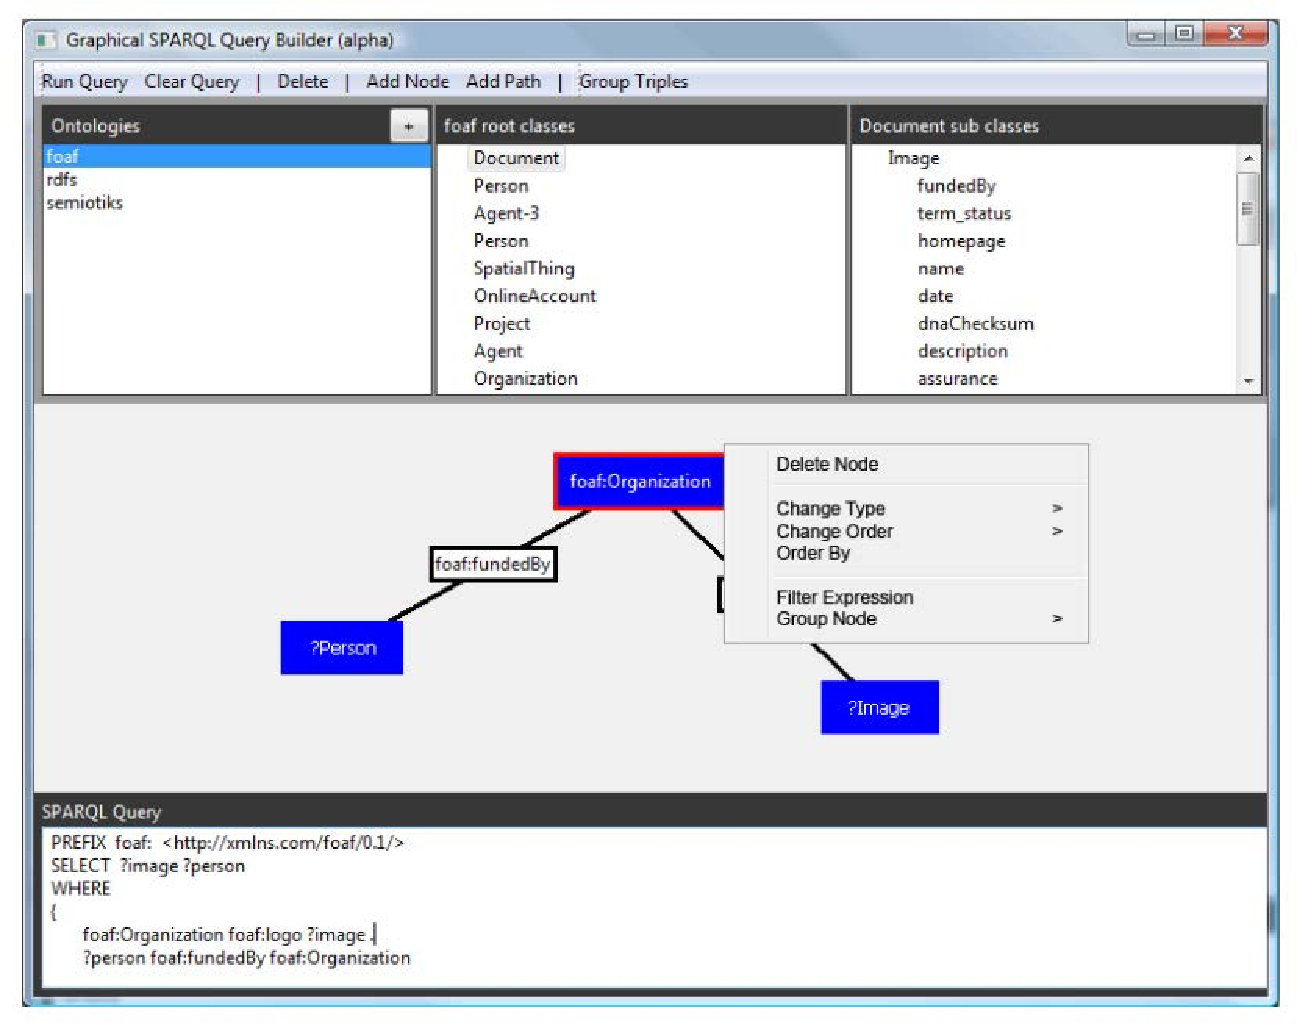
\includegraphics[width=.9\linewidth]{NitelightFigure1.pdf}
  \caption{An overview of the Nitelight user interface\cite{Nitelight}}
  \label{fig:NitelightUI}
\end{figure}
\\
Figure \ref{fig:NitelightUI} is an image of Nitelight in action. Nitelight is developed as a Java application and has some different tools to use. In the top it has basic commands such as running the query and adding new nodes. Below is the ontology browser, which can be used for the user to look through the different ontologies and what they consist of. Under the ontology browser is the node view, which is the main part of Nitelight. Here the nodes are set up in such a way that shows their relation to each other and this all results in the SPARQL query in the bottom. This text view is the result of the visual query and is read only.
\\\\
To elaborate on how the node view represents the finished query, use figure \ref{fig:NitelightBreakDown} for reference. Here it is shown that the query deals with three parts, the bound variable, the unbound variable and the literal predicate. The unbound variable points to the literal predicate, which then points to the bound variable. An example of this can also be seen in figure a, where a person (the bound variable) is funded by (the literal predicate) an organisation (unbound variable).

\begin{figure}[h]
    \centering
  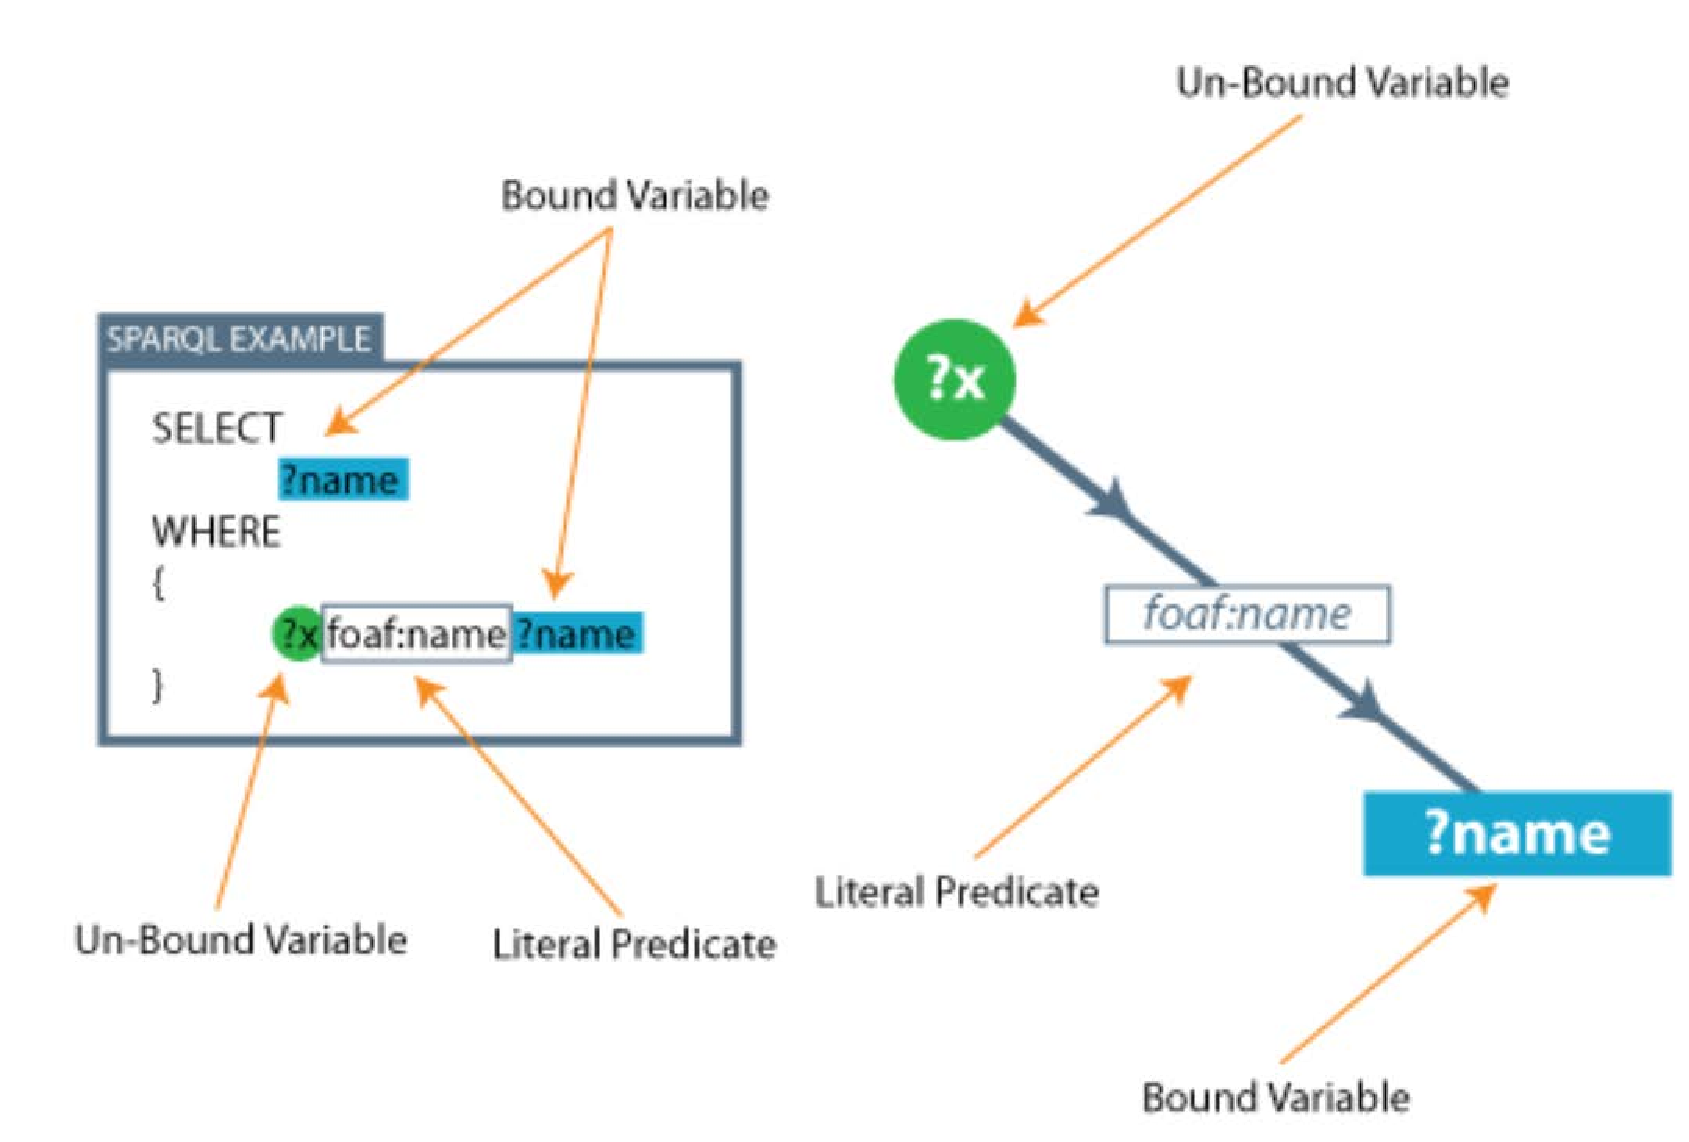
\includegraphics[width=.9\linewidth]{NitelightFigure2.pdf}
  \caption{Breaking down SPARQL queries to visualization\cite{Nitelight}}
  \label{fig:NitelightBreakDown}
\end{figure}

\subsection{QueryVOWL}
QueryVOWL is a visual query language to help users develop SPARQL queries\cite{QueryVOWL}, similarly to Nitelight. It is however developed as a webcomponent using HTML, CSS, JavaScript and SVG. It has three views, the main visual view, the sidebar for additional options and a result list containing the SPARQL query. The main view implements a drag and drop interface, which results in a completed SPARQL query without the need for the user to know perfect syntax. It can take any RDF dataset containing SPARQL endpoints.

\subsection{SPARQL-visualizer: A Communication Tool for Collaborative Ontology Engineering Processes}
This is a visualisation of the query result\cite{MadsHoltenSPARQL} and not the query itself. Therefore it could seem less relevant, however the way the graphical elements are implemented is something that can be used as inspiration. This leads to the library D3.js, a graphics library in JavaScript. The paper references (https://github.com/Rathachai/d3rdf) as a way to create a force layout of D3.js to visualize the expression "subject–predicate–object".



\section{Approach}
The solution will consist of a webcomponent, using JavaScript, that has two views for composing SPARQL queries, a textual and a visual. The visual view will be processed through SVG and should come in the form of a spring graph model layout. The user can interact with the visualisation through a drag and drop interface. The visualisation will then affect the textual view by writing the query in text. Likewise, will the visual view be affected by the textual view. Lastly, the visualisation has the option to be saved locally.

\section{Project goals}
The goals for this project are:
\begin{enumerate}
    \item To learn about RDF and SPARQL.
    \item To make a tool for visualising SPARQL queries.
    \item To make it easy to visualise and convert between a graphical and textual view of a SPARQL query.
\end{enumerate}

\section{Report structure}
{\color{red}missing\\}